\chapter{Integer Linear Programming}
\section{Introduction}

The setting is very similar to the linear programs we already know. We just restrict the problems and the possible solutions a bit. As the name suggests we want integer solutions to our programs. That means we should have an integer constraint matrix too. 

\begin{Def}[Integere Linear Program] Given $A\in \Z^{m\times n}$, $b\in \Z^m$, $c\in \Z^{1\times n}$ find a $x\in \Z^n$ such that $Ax\leq b$ and $cx$ is maximal (or minimal)

\begin{align*}
\max \quad & cx \\
s.t. \quad & Ax \leq b\\
&x\in \Z^n
\end{align*}
\end{Def}

If we just restrict some variables to be integral we have a mixed integer linear program.

Integer linear programs allow us to model some new interesting problems that we couldn't before. The most prominent examples are 

\begin{itemize}
\item binary choices, e.g. many NP-complete problems like Knapsack require some choice. 
\item relations between variables, e.g. choose at most ten of these things $\sum x_i \leq 10, x_i\in \{0,1\}$
\item disjunctive constraints, e.g. $x\geq a$ or $y\geq b$, can be modeled by introducing a decision variable $\delta \in \{0,1\}$ and saying $x\geq a\delta$ and $y \geq b(1-\delta)$. 
\item conditional constraints, e.g. if $x>a$ then $y>b$, can be modeled using disjunctive constraints: $x\leq a$ or $y>b$
\item piecewise linear cost functions become possible by introducing decision variables that decide on the piece we're in.
\end{itemize}

Integer Linear Programs are harder to solve than normal linear programs. Rounding, for example, doesn't work very well, as the cost difference between the optimal integral solution and an optimal fractional solution can be quite large.

\begin{thm} Finding a feasible solution for an ILP is NP-complete.
\end{thm}

\begin{pr} We prove by a reduction from SAT that ILP is NP-hard. For a given formula in CNF we construct an ILP like this:

For each variable $v_j$ in the formula we introduce $z_j \in \{0,1\}$ in our ILP, with the natural interpretation of the value of $z_j$. For every clause $C_i$ let $J^+_i$ be the number of positive and $J^-_i$ be the number of negated variables in clause $C_i$.

The ILP for the formula is then

\begin{align*}
\max \quad & 42 \\
s.t. &\sum_{j\in J^+_i} z_j + \sum_{j\in J^-_i} (1-z_j) \geq 1 && \forall i\\
&z_j \in \{0,1\}
\end{align*}

The constraints make sure that in every clause at least one positive variable is 1 or one negative variable is 0. If the feasible region of the LP is nonempty then the formula is satisfiable. The formal proof is omitted as it is rather obvious.

To show NP completeness we need to show that ILP is in NP. In the 0-1 case it is rather obvious that we can use any feasible solution as a polynomial witness. In the general case we would need to show that the entries in the solution vector are polynomially bounded. This is quite complicated but follows from the ellipsoid method. We will omit that proof here.
\end{pr}

NP-completeness is a worst-case statement. Some ILPs can be solved efficiently. We'll talk about conditions for that.

\section{Integer hull of a polyhedron}

The integer hull of a polyhedron is the set of feasible solutions $\{x | Ax\leq b, x\in \Z^n\}$. As we know $\{x|Ax\leq b\}$ is a polyhedron. Let $P_I = \{x| Ax\leq b\}_I$ be the convex hull of the integral vectors in $P$. See figure \ref{Fig:integerHull}

\begin{figure}[hbt]
\begin{center}
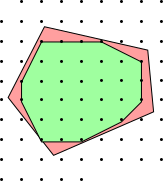
\includegraphics{./images/integerHull}
\end{center}
\caption{The integer hull of a polyhedron}
\label{Fig:integerHull}
\end{figure}

We make the following propositions:

\begin{enumerate}
\item If $P$ is bounded then so is $P_I$
\item If $A$ contains only rational numbers, $P$ is rational. For rational $P$ the integer hull is also a polyhedron.
\item If $P$ is unbounded and $A,b$ arbitrary real then $P_I$ is not necessarily a polyhedron.
\end{enumerate}

Obviously if $P=P_I$ then the solution for an ILP with feasible region $P_I$ is the same as the solution for the relaxed problem with feasible region $P$.

\begin{Def} A polyhedron $P$ is called integral if $P=P_I$\end{Def}

\begin{thm}\label{Thm:polyIntegrality} A rational polyhedron $P$ is integral iff

\[\max \{cx | x\in P\}\in \Z\quad \forall c\in \Z^{1\times n}\]

and the maximum is finite.
\end{thm}

\begin{pr} If the polyhedron is integral any optimal solution will also be integral, so that direction is easy.

For the other direction suppose $\max \{cx | x\in P\}\in \Z\quad \forall c\in \Z^{1\times n}$. Let $y\in P$ be a unique optimal solution for $c$. We have 

\[cy>cx + x_1 -y_1 \quad \forall x\in P,x\neq y\]

By multiplying $c$ be an arbitrary integer we can make the gap between the unique optimal solution $y$ and any other solution $x$ as large as we want, in particular large enough to make that inequality true.

We can change the cost function a bit without making $y$ nonoptimal. Let $\bar c = (c_1+1,c_{2,\ldots,n})$. 

\[\bar c y > \bar c x\qquad \forall x\neq y\]

We want to compute by how much the cost did change. Since we increased the first component of $c$ we get

\[\bar c y = cy+y_1\]

Since we assumed that $cy$ is integral and our modification didn't change didn't change that integrality that equality forces $y_1$ to be integral too. We can do that for all components so they must all be integral. Since this must hold for all cost vectors it holds for all vertices and our polyhedron must be integral.
\end{pr}

Now we want to recognise integral polyhedra by looking at the constraint matrix. 

\section{Total dual integrality}

Strong duality as for linear programs does not hold for ILPs. But we have something similar

\begin{Def} A system $Ax\leq b$ is called totally dual integral (TDI) if for each integral $c$ with bounded maximum we have

\[\max \{cx |Ax\leq b\} = \min \{\trans y b | \trans y A = \trans c, y\geq 0, y\in \Z^m\}\]

Note that $x$ doesn't have to be integral here.

The same works for $Ax\leq b, x\geq 0$ and $Ax=b, x\geq 0$
\end{Def}

Notable here is that TDI is not a property of the polyhedron but instead of the system that defines it. Very much like with degeneracy we may find another system that describes the same polyhedron but is in fact TDI.

This together with theorem \ref{Thm:polyIntegrality} has the following corollary: Let $A\in \Q^{n\times m}$, $b\in \Z^n$ and $Ax\leq b$ is TDI then $\{x|Ax\leq b\}$ is integral.

This condition is checkable, but we don't really know how to use it yet.

\begin{Ex} Given a directed graph $G=(V,E)$, two vertices $s,t\in V$ and the set of pathes between $s,t$. We're also given a cost function $c$ on the edges. The task is to assign positive weights $y_e$ to the edges s.t. each path has accumulated cost at least 1. While doing so we want to minimize

\[\sum_{e\in E} c(e), y_e\]

Formulated as a LP that is 

\begin{align*}
\min \quad & \sum_{e\in E} c(e) y_e\\
s.t. & \sum_{e\in p} y_e \geq 1 && \forall p\in P\\
&y_e \geq 0
\end{align*}

We want to show that the polyhedron $Q$ that is defined be the above constraints is integral by showing that it is TDI. To do that we construct the dual:

\begin{align*}
\max \quad & \sum_{p\in P} x_p\\
s.t. & \sum_{p,e\in P} x_p \leq c(e) && \forall e\in E\\
 & x_p \geq 0 && p\in P
\end{align*}

By looking hard at the dual we see that it defines a maximum flow problem. As we know maximum flow problems with integer capacities have integral optimal solutions. Hence we have a TDI system.
\end{Ex}